\documentclass[a4paper,
fontsize=11pt,
%headings=small,
oneside,
numbers=noperiodatend,
parskip=half-,
bibliography=totoc,
final
]{scrartcl}

\usepackage{synttree}
\usepackage{graphicx}
\setkeys{Gin}{width=.4\textwidth} %default pics size

\graphicspath{{./plots/}}
\usepackage[ngerman]{babel}
\usepackage[T1]{fontenc}
%\usepackage{amsmath}
\usepackage[utf8x]{inputenc}
\usepackage [hyphens]{url}
\usepackage{booktabs} 
\usepackage[left=2.4cm,right=2.4cm,top=2.3cm,bottom=2cm,headheight=25.60228pt,includeheadfoot]{geometry}
\usepackage{eurosym}
\usepackage{multirow}
\usepackage[ngerman]{varioref}
\setcapindent{1em}
\renewcommand{\labelitemi}{--}
\usepackage{paralist}
\usepackage{pdfpages}
\usepackage{lscape}
\usepackage{float}
\usepackage{acronym}
\usepackage{eurosym}
\usepackage[babel]{csquotes}
\usepackage{longtable,lscape}
\usepackage{mathpazo}
\usepackage[flushmargin,ragged]{footmisc} % left align footnote

%%url brekas grrr
\def\UrlBreaks{\do\a\do\b\do\c\do\d\do\e\do\f\do\g\do\h\do\i\do\j\do\k\do\l%
\do\m\do\n\do\o\do\p\do\q\do\r\do\s\do\t\do\u\do\v\do\w\do\x\do\y\do\z\do\0%
\do\1\do\2\do\3\do\4\do\5\do\6\do\7\do\8\do\9\do\-}%

\usepackage{listings}

\urlstyle{same}  % don't use monospace font for urls

\usepackage[fleqn]{amsmath}

%adjust fontsize for part

%% geometry
\clubpenalty = 10000 
\widowpenalty = 10000 
\displaywidowpenalty = 10000
%% tightlist

\providecommand{\tightlist}{%
  \setlength{\itemsep}{0pt}\setlength{\parskip}{0pt}}

\usepackage{sectsty}
\partfont{\large}

%Das BibTeX-Zeichen mit \BibTeX setzen:
\def\symbol#1{\char #1\relax}
\def\bsl{{\tt\symbol{'134}}}
\def\BibTeX{{\rm B\kern-.05em{\sc i\kern-.025em b}\kern-.08em
    T\kern-.1667em\lower.7ex\hbox{E}\kern-.125emX}}

\usepackage{fancyhdr}
\fancyhf{}
\pagestyle{fancyplain}
\fancyhead[R]{\thepage}

%meta

%meta

\fancyhead[L]{T.C. Kim \& P. Zumstein \\ %author
LIBREAS. Library Ideas, 29 (2016). % journal, issue, volume.
\href{http://nbn-resolving.de/urn:nbn:de:kobv:11-100238157
}{urn:nbn:de:kobv:11-100238157}} % urn
\fancyhead[R]{\thepage} %page number
\fancyfoot[L] {\textit{Creative Commons BY 3.0}} %licence
\fancyfoot[R] {\textit{ISSN: 1860-7950}}

\title{\LARGE{Semiautomatische Katalogisierung und Normdatenverknüpfung mit Zotero im Index Theologicus}} %title %title
\author{Timotheus Chang-whae Kim \& Philipp Zumstein} %author

\setcounter{page}{}

\usepackage[colorlinks, linkcolor=black,citecolor=black, urlcolor=blue,
breaklinks= true]{hyperref}

\date{}
\begin{document}

\maketitle
\thispagestyle{fancyplain} 

%abstracts
\begin{abstract}
\small
\textbf{Zusammenfassung:} Im Folgenden soll aufgezeigt werden, wie
derzeit das Literaturverwaltungsprogramm Zotero innerhalb des Index
Theologicus genutzt wird, um unselbstständige Literatur in einem
bibliothekarischen Katalogisierungssystem zu erfassen. Die modulare und
flexible Architektur der Open Source Software erlaubt es, die bereits
kollaborativ zusammengetragene Programmierarbeit zur Datenextraktion
mitzunutzen. Das vorgestellte semiautomatische Verfahren bringt auch bei
der Verknüpfung von Normdaten erhebliche Vorteile für die
Medienbearbeitung.

\textbf{Schlüsselwörter:} Literauturverwaltungsprogramm, Zotero,
Katalogisierung, Unselbständige Werke, Aufsatzliteratur, Index
Theologicus, Online-Bibliographie, WinIBW, Fachinformationsdienst
Theologie

\begin{center}\rule{0.5\linewidth}{\linethickness}\end{center}

\textbf{Abstract:} This article presents an approach to use the
reference management software Zotero within the theological article
database Index Theologicus to catalogue article metadata for a library
management system. Zotero's Open Source nature and flexible architecture
allowed us to seamlessly reuse the vast amount of data extraction
routines collaboratively developed for the software. We will show how
the semi-automatic workflow we developed will make authority linking fun
again.

\textbf{Keywords:} Reference Management System, Zotero, Cataloguing,
Journal articles, Index Theologicus, Theological database, Academic
Information Services for Theology
\end{abstract}

%body
Eine traditionelle Aufgabe von Bibliotheken ist es, relevante Literatur
zu erschließen und für die Recherche nutzbar zu machen. Dabei
konzentrierte sich die Katalogisierungsarbeit in Bibliotheken meist auf
Monographien, Sammelwerke oder die Gesamtaufnahmen von Zeitschriften,
ohne die darin enthaltenen Artikel auszuwerten. Eine Ausnahme stellt der
Index Theologicus (IxTheo)\footnote{\url{https://www.openhub.net/}} der
Universitätsbibliothek Tübingen dar.

Der IxTheo geht zurück auf die 1975 als gedruckter
Zeitschrifteninhaltsdienst Theologie begonnene Aufsatzdokumentation und
erscheint seit 2007 nur noch online als frei zugängliche
Aufsatzdatenbank (\enquote{Zur Geschichte des Index theologicus}, 2007).
Bis dato ist der IxTheo eine der wichtigsten und frei zugänglichen
bibliographischen Datenbanken im Bereich Theologie und
Religionswissenschaft, die umfassend theologische Aufsatzliteratur
dokumentiert. Zudem wird der IxTheo im Rahmen des
Fachinformationsdienstes (FID) Theologie\footnote{\url{http://www.ub.uni-tuebingen.de/fidtheo}}
2016 zu einer umfassenden, wissenschaftlichen Bibliographie für
Theologie und Religionswissenschaft ausgebaut, in der neben
unselbständiger auch selbständige Literatur sowie Datenbanken und
ausgewählte Internetlinks nachgewiesen werden.

Andere frei zugängliche theologische Spezialbibliographien wie

\begin{itemize}
\item
  die Bibelwissenschaftliche Literaturdokumentation Innsbruck
  (BILDI\footnote{\url{https://www.uibk.ac.at/bildi/index.html.de}}),
\item
  die Analytische Bibliographie zum Deuteronomium (AnaBiDeut),
\item
  die Bibliographie biblique informatisée de Lausanne (BiBIL),
\item
  der Catalogue de l'École Biblique et Archéologique Française in
  Jerusalem (CEBAF\footnote{\url{http://www.ebaf.edu/wp-content/uploads/biblio/en-aide-all.pdf}},
\item
  die Missionsbibliothek und katholische Dokumentationsstelle
  (MIKADO\footnote{\url{http://www.mikado-ac.info/home.html}}),
\item
  die Kanonistische Literaturdokumentation Innsbruck (KALDI\footnote{\url{https://www.uibk.ac.at/praktheol/kaldi/}}),
\item
  die Datenbank zur mimetischen Theorie von René Girard
  (MIMESI\footnote{\url{https://www.uibk.ac.at/rgkw/drama/mimdok/index.html.de}})
  und
\item
  der Theologische Schlagwortkatalog für Genderforschung (TSG\footnote{\url{http://www.netzwerk-fgf.nrw.de/fileadmin/media/media-fgf/download/publikationen/Journal-33_Netzwerk_FGF.pdf}})
\end{itemize}

sind auf eine bestimmte theologische Teildisziplinen spezialisiert und
decken -- anders als der IxTheo -- nicht alle theologischen Disziplinen
umfassend ab.

Um aber eine solche freie bibliographische Datenbank dauerhaft betreiben
und weiterentwickeln zu können, sind neben solider Infrastruktur
zunehmend stärkere Vernetzung und Kooperation in Form von Informations-
und Datenaustausch untereinander erforderlich. Vor allem sollten die
Metadaten idealerweise arbeitsteilig in einem standardisierten
Datenformat von den kooperierenden Einrichtungen gemeinsam hergestellt
werden. Softwaretools sollten den Datenerfassenden ihre Tätigkeit so
einfach wie möglich machen und einzelne Arbeitsschritte weitgehend
automatisieren.

Eine Herausforderung bei der Aufsatzkatalogisierung in einer
Verbundumgebung ist jedoch die um Größenordnungen höhere Zahl von zu
bearbeitenden Aufnahmen und damit einhergehend die Problematik
zeitintensiver Bearbeitung der Normdaten. Softwaregestützte
semiautomatische Verfahren können auch bei dieser Problematik Abhilfe
schaffen, wie wir anhand von Zotero zeigen wollen.

\section*{Katalogisierung im Index
Theologicus}\label{katalogisierung-im-index-theologicus}

Seit 2013 wird die unselbständige Literatur nicht mehr in der
allegro-Datenbank, sondern direkt im Pica-CBS des Südwestdeutschen
Bibliotheksverbundes (SWB) erfasst. Die Migration der circa 507.000
\enquote{Altdaten} in die SWB-Datenbank ist dieses Jahr erfolgt und
demnächst wird noch der jetzige IxTheo-Katalog durch ein modernes
Resource Discovery System (\emph{Vufind)} abgelöst. Seitdem die
Katalogisierung im SWB-Verbund erfolgt, ist die Normdatenverknüpfung und
-erstellung der Autoren in der gemeinsamen Normdatei (GND) als neue,
aufwändige Aufgabe hinzugekommen.

Mit großem Engagement des früheren und jetzigen IxTheo-Teams konnten
bislang mit konventionellen Methoden im IxTheo circa 12.000-20.000
Aufsätze jährlich ausgewertet und mit Schlagwörtern und
IxTheo-Klassen\footnote{\url{http://web.archive.org/web/20160413144655/http://www.ixtheo.de/klassger.htm}}
analytisch tief erschlossen werden. Im Zuge der erfolgreichen
Überführung vom Sondersammelgebiet (SSG) in den Fachinformationsdienst
(FID) Theologie soll der Zeitschriftenkanon des IxTheo über die rund 600
laufend ausgewerteten Zeitschriften hinaus deutlich ausgeweitet werden.
Dabei setzen wir neben der automatischen Dateneinspielung von
Verlagsdaten (zum Beispiel von DeGruyter) auch das neue semiautomatische
Produktionsverfahren mittels Zotero u.a bei der Gewinnung der Metadaten
ein. Von den ungefähr 1.800 laufenden Zeitschriftenabonnements aus den
Beständen des SSG/FID Theologie und Religionswissenschaft der UB
Tübingen können vor allem Zeitschriften, die nur noch online erscheinen,
unter Einsatz von Zotero im Katalogisierungsclient WinIBW katalogisiert
werden.

Die mit diesem neuen Verfahren hergestellte Metadaten werden dann aus
der SWB-Ver\-bund\-daten\-bank exportiert und im Solr-Index des IxTheo
indexiert. Diese sichere und dauerhafte Datenhaltung in der
SWB-Ver\-bund\-daten\-bank erleichtert die Nachnutzung der Daten sowie
Kooperationsbestrebungen mit anderen Bibliotheken, die den WinIBW als
Katalogisierungsclient nutzen (Faßnacht 2015).

\section*{Zotero Translators zur
Datenextraktion}\label{zotero-translators-zur-datenextraktion}

Zotero\footnote{\url{https://www.zotero.org/}} ist eine
Literaturverwaltungssoftware, welche als Open Source Software vom Roy
Rosenzweig Center for History and New Media der George Mason University
zusammen mit der Zotero-Community entwickelt wird. Als Programm zur
Literaturverwaltung integriert sich Zotero in den wissenschaftlichen
Schreibprozess, unterstützt beim Aufbau und der Verwaltung einer
persönlichen Literaturdatenbank und vereinfacht es, die Angaben bei
Belegstellen in Zitationen sowie das Quellenverzeichnis zu erstellen.
Die primäre Zielgruppe für das Programm sind somit alle, die
wissenschaftlich schreiben und publizieren müssen, wie etwa Forschende
oder Studierende. Auch in Deutschland bieten viele Bibliotheken Kurse
zur Nutzung von Zotero und anderen Literaturverwaltungsprogrammen an.

Eine wesentliche Funktionalität ist die einfache und komfortable
Integration in den Webbrowser, um die eigene Literaturdatenbank gleich
bei Recherche im Web zu füllen. Dies geschieht in Zotero vor allem über
den \emph{Zotero-Speichern-Button (Zotero-Picker)}, mit welchem man mit
einem Klick die bibliographischen Metadaten der aktuellen Webseite
extrahieren und speichern kann. Daneben gibt es auch noch weitere
Möglichkeiten wie etwa das Im\-portieren von bibliographischen Metadaten
oder das Suchen nach bestimmten Identifikatoren mit dem
\enquote{\emph{Zauberstab}}. Diese drei Funktionalitäten zusammen mit
den Export-Möglichkeiten werden über sogenannte Zotero
Translators\footnote{\enquote{Zotero Übersetzer}:
  \url{https://www.zotero.org/support/dev/translators}} bereitgestellt
wie in Abb. 1 dargestellt ist.

\begin{figure}[htbp]
\centering
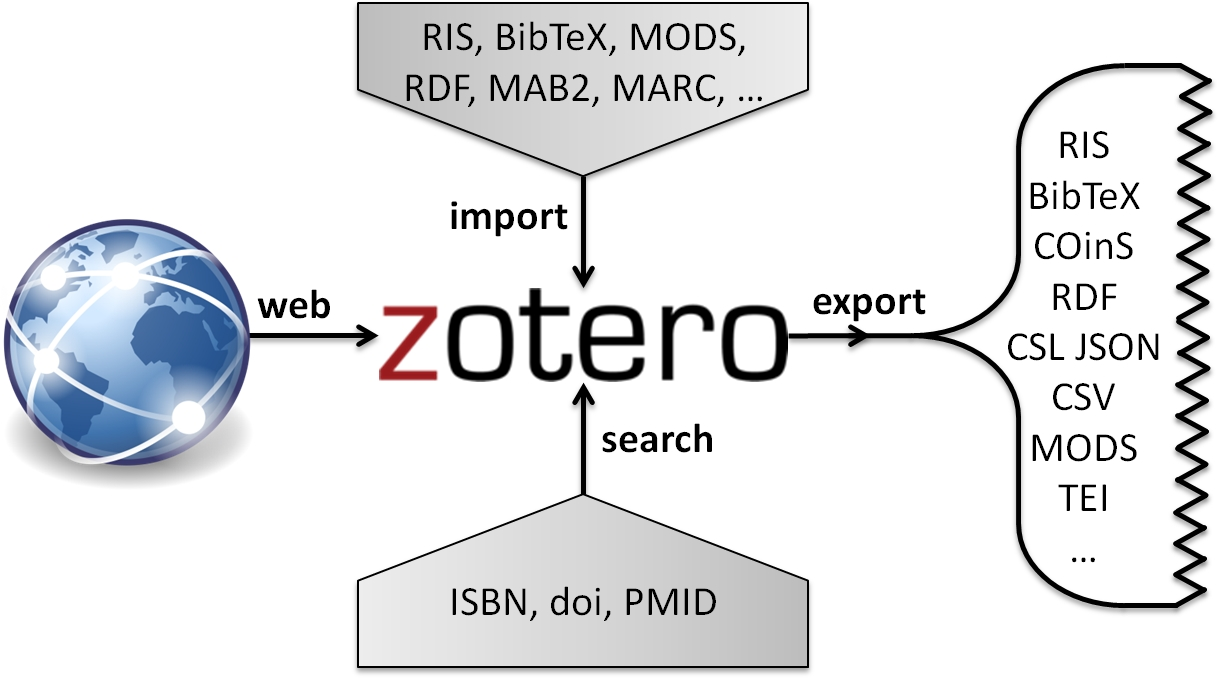
\includegraphics{img/Zotero-Translators.jpg}
\caption{Die vier verschiedenen Typen von Zotero translators (web,
im\-port, search, export) mit Beispielen}
\end{figure}

Zotero kann ähnlich einem Simultanübersetzer (oder
{[}Babelfisch\footnote{\url{https://de.wikipedia.org/wiki/Babelfisch}})
agieren und zwischen verschiedenen Datenformaten übersetzen.
Beispielsweise ist es mit Zotero über entsprechende Im\-port- sowie
Export-Schritte möglich, MARC-Daten zusammen mit MODS-Daten in einer
gemeinsamen CSV-Datei auszugeben. Für solche oder ähnliche
Transformationsschritte gibt es aber auch spezialisiertere Tools aus dem
Bereich Metadatenmanagement (siehe Pfeffer 2016).

Wohl einzigartig sind aber die Möglichkeiten, strukturierte Metadaten
aus einer Vielzahl von bibliographischen Webseiten zu extrahieren, mit
Hilfe des Zotero Web Translators. Es gibt etwa 440 Web Translators
(Stand April 2016), die aus der Präsentationsschicht von Verlagen,
Bibliotheken, Digitalen Archiven, Zeitschriften et cetera die
bibliographischen Metadaten generieren. Häufig werden bei diesen
Webseiten die Maschinenlesbarkeit beispielsweise für
Literaturverwaltungsprogramme, Export-Möglichkeiten in Standardformate
und die Pflege guter APIs zugunsten einer hübschen Präsentation
vernachlässigt (Zumstein \& Stöhr 2015). Daher müssen Web Translators
die Informationen häufig aus den Webseiten \enquote{herauskratzen} (web
scraping). Somit sind Zotero Translators vielfach die einzige
Möglichkeit, ohne großen Aufwand bibliographische Daten automatisiert
aus bestimmten Webseiten zu extrahieren.

Das Translator Framework ist modular, das heißt jeder Translator ist
eine eigene Javascript-Datei mit Metadaten und Testfällen. Wir haben
zokat\footnote{\url{https://github.com/UB-Mannheim/zotkat}}, eine
Erweiterung für den Einsatz von Zotero bei der Katalogisierung, als Open
Source entwickelt. Eine zentrale Komponente von zotkat ist ein Export
Translator für das Pica3-Format des SWB, das für IxTheo eingesetzt wird.
Durch die Hinzunahme dieses einen Translators für den Export können für
eine Unmenge von Webseiten die bibliographischen Daten extrahiert und im
Katalogisierungsclient genutzt werden. Der praktische Ablauf wird im
nächsten Abschnitt beschrieben.

Alternativ könnte man, um Artikel von einer einzelnen Webseite zu
extrahieren, natürlich auch eine eigene Lösung programmieren, aber dies
ist einerseits nur begrenzt möglich und scheint häufig über den eigenen
Gebrauch hinaus keinen Nutzen zu bringen. Dahingegen schafft die
Verwendung eines einheitlichen Frameworks Synergieeffekte und ist für
viele verschiedene Anwendungsfälle nachhaltig. Mehr als 65 Personen
haben sich an der Entwicklung von Zotero Translators bereits beteiligt.
Dabei sind etwa 480 Translators kollaborativ entstanden und werden von
der Community gepflegt sowie weiterentwickelt. Dies entspricht insgesamt
etwa 117.000 Zeilen Code,\footnote{Es wurden 116.983 Codezeilen eruiert
  mit dem Tool \url{https://github.com/AlDanial/cloc} am 29.03.2016.}
was nach dem COCOMO Modell\footnote{\url{https://de.wikipedia.org/wiki/COCOMO}}
etwa 30 Personenjahren\footnote{Wir verwenden die gleichen Parameter wie
  bei bei \url{https://www.openhub.net/}, d.h. a=2,4, b=1,04 bei PM =
  a*KDSI\^{}b, wobei KDSI die Anzahl von auszuliefernden Codezeilen in
  Tausend entspricht} Entwicklungszeit entsprechen würde. Die Zotero
Translators werden auch von Wikipedia innerhalb von Citoid\footnote{\url{https://www.mediawiki.org/wiki/Citoid}}
verwendet und ProQuest nutzt sie in PME\footnote{\url{https://github.com/proquest/PME}}
nach.

\section*{Katalogisierungsworkflow in der
Praxis}\label{katalogisierungsworkflow-in-der-praxis}

Zur Illustration des Katalogisierungsworkflow in der Praxis, welchen wir
hier im Folgenden beschreiben, haben wir noch ein kurzes Video (ohne
Ton) erstellt\footnote{\url{https://bibserv24.bib.uni-mannheim.de/owncloud/index.php/s/oLAXTm9yBaqHaVc}}.

Nach der Installation von Zotero als Add-on im Firefox-Browser werden
über den Zotero-Picker in der Symbolleiste die bibliographischen
Metadaten aus verschiedenen Datenquellen wie Verlagswebseiten,
Fachdatenbanken, OA-Journals und Bibliothekskatalogen et cetera in
\enquote{Meine Bibliothek} heruntergeladen. Dabei kann je nach Webseite
zwischen unterschiedlichen Downloadoptionen gewählt werden (Einzel- und
Mehrfachübernahmen, Persistente Identifikatoren mittels
``*Zauberstab``*, Im\-portfunktion von anderen Formate). In den meisten
großen Aufsatzdatenbanken wie JSTOR oder EBSCO ist Mehrfachübernahme,
das hißt alle Aufsätze eines Zeitschriftenheftes mit einem Klick,
möglich.

\begin{figure}[htbp]
\centering
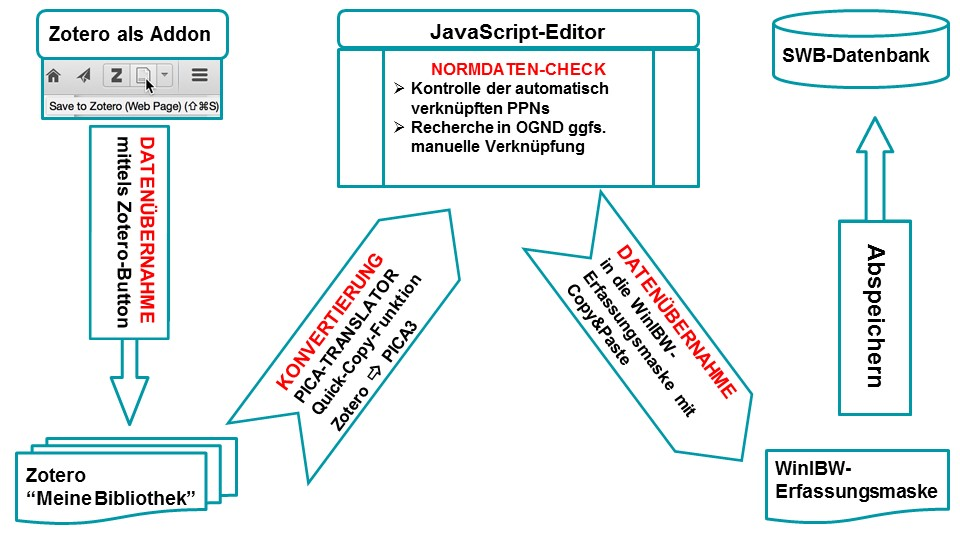
\includegraphics{img/Workflow.jpg}
\caption{Katalogisierungsworkflow}
\end{figure}

Da die heruntergeladenen Metadaten desselben Aufsatzes je nach
Download-Option variieren, muss einmal vorher überprüft werden, welche
Option die optimalen Metadaten für die Katalogisierung liefert. Um die
Bearbeitung einer \enquote{Zotero-geeigneten} Zeitschrift im
IxTheo-Geschäftsgang zu erleichtern, tragen wir Informationen wie das
Produktionsverfahren, Datenquelle mit Permalink, die zu wählende
Downloadoption und andere in einem internen Zeitschriftenverwaltungstool
zusammen.

Die im Zotero-Ordner gespeicherten Metadaten werden dann einzeln mit
Copy \& Paste oder Drag \& Drop in einen
\href{http://www.w3schools.com/js/tryit.asp?filename=tryjs_myfirst}{\emph{JavaScript-Editor}}
eingefügt und anschließend im rechten \enquote{Result}-Fenster (Abb.3)
die automatisch erzeugte Autoren-SWB-PPN intellektuell kontrolliert. Für
die leichte Kontrolle und eventuelle Nachverknüpfung der PPN werden
zusätzlich zwei Links\footnote{Link 1:
  \textless{}http://swb.bsz-bw.de/DB=2.104/SET=1/TTL=1/CMD?SGE=\&ACT=SRCHM\&MATCFILTER=Y\&MATCSET=Y\&NOSCAN=Y\&PARSE\_MNEMONICS=N\&PARSE\_OPWORDS=N\&PARSE\_OLDSETS=N\&IMPLAND=Y\&NOABS=Y\&ACT0=SRCHA\&SHRTST=50\&IKT0=1004\&TRM0=Berger,
  Klaus\&ACT1=\emph{\&IKT1=2057\&TRM1=3.}\&ACT2=*\&IKT2=8991\&TRM2=19**\&ACT3=\%2B\&IKT3=4060\&TRM3=tpv\emph{\&ACT4=\%2B\&IKT4=8991\&TRM4=theol}
  neutestament\emph{\&ACT5=}\&IKT5=1004\&TRM5=Berger,
  Klaus\textgreater{}, Link 2:
  \textless{}http://swb.bsz-bw.de/DB=2.104/SET=1/TTL=1/CMD?SGE=\&ACT=SRCHM\&MATCFILTER=Y\&MATCSET=Y\&NOSCAN=Y\&PARSE\_MNEMONICS=N\&PARSE\_OPWORDS=N\&PARSE\_OLDSETS=N\&IMPLAND=Y\&NOABS=Y\&ACT0=SRCHA\&SHRTST=50\&IKT0=1004\&TRM0=Berger\&ACT1=\emph{\&IKT1=2057\&TRM1=3.}\&ACT2=*\&IKT2=8991\&TRM2=19**\&ACT3=\%2B\&IKT3=4060\&TRM3=tpv\emph{\&ACT4=\%2B\&IKT4=8991\&TRM4=theol}
  neutestament\emph{\&ACT5=}\&IKT5=1004\&TRM5=Berger\textgreater{}} mit
unterschiedlich vordefinierten Suchabfragen automatisch erzeugt, deren
Ergebnis im rechten \enquote{Result}-Fenster direkt angeklickt und
angezeigt werden kann. (Abb. 3)

\begin{figure}[htbp]
\centering
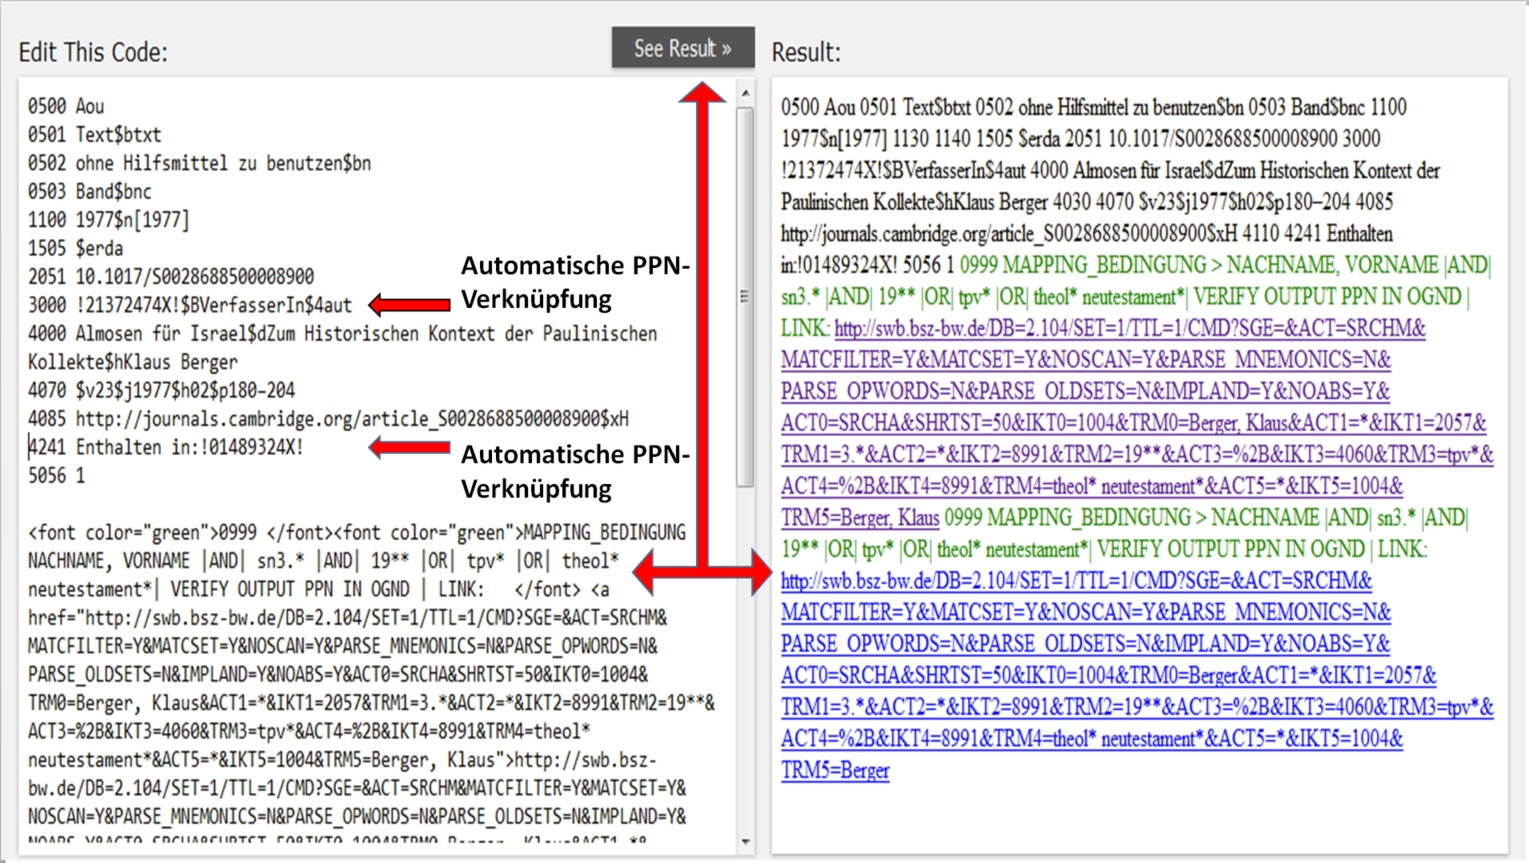
\includegraphics{img/Normdatenkontrolle.jpg}
\caption{Ansicht für die Normdatenkontrolle und -recherche}
\end{figure}

Die Verknüpfungen mit den Normdaten werden auf unterschiedliche Weise
realisiert. Die bekannten Zeitschriften der Theologie sowie eine Liste
von Autoren wurden im Vorfeld zusammen mit der SWB-PPN in einer
Mapping-Tabelle hinterlegt. Jedes Mal wenn bei einem Aufsatz der
Zeitschriftentitel oder Autorenname in dieser Liste vorkommt, wird
dieser Text beim Export mit dem Pica3-Translator durch die entsprechende
Normdatenverknüpfung (PPN) ersetzt. Zusätzlich werden bei den Autoren
auch noch zwei Links im Pseudo-Pica-Felder 0999 erzeugt. Diese Links
fragen die Namensform \enquote{Nachname, Vorname} verbunden mit weiteren
spezifizierten Suchattributen wie Berufsbezeichnung (\enquote{theol*},
\enquote{bischof*}, \enquote{pfarr*}), GND-Systematik (\enquote{3.*})
und Lebensdaten (\enquote{19xx}) ab, um ein möglichst eindeutiges
Mappingergebnis zu erzielen. Diese OGND-Suchabfrage kann zudem
projektspezifisch
\href{https://github.com/UB-Mannheim/zotkat/wiki/Suche-nach-Autoren-Normdaten-im-Online-GND-(OGND)-Katalog}{\emph{weiter
angepasst}} werden. Diese Links dienen einerseits der Kontrolle, können
aber auch weiter zur Recherche bei verschiedenen Personen mit dem
gleichen Namen benutzt werden (Abb. 4). Nach diesem Arbeitsschritt kann
dann die Pica3-Titelaufnahme ohne die Links aus dem linken Fenster
wieder in die Erfassungsmaske der WinIBW mit Copy \& Paste übernommen
und in der Regel direkt abgespeichert werden.

\begin{figure}[htbp]
\centering
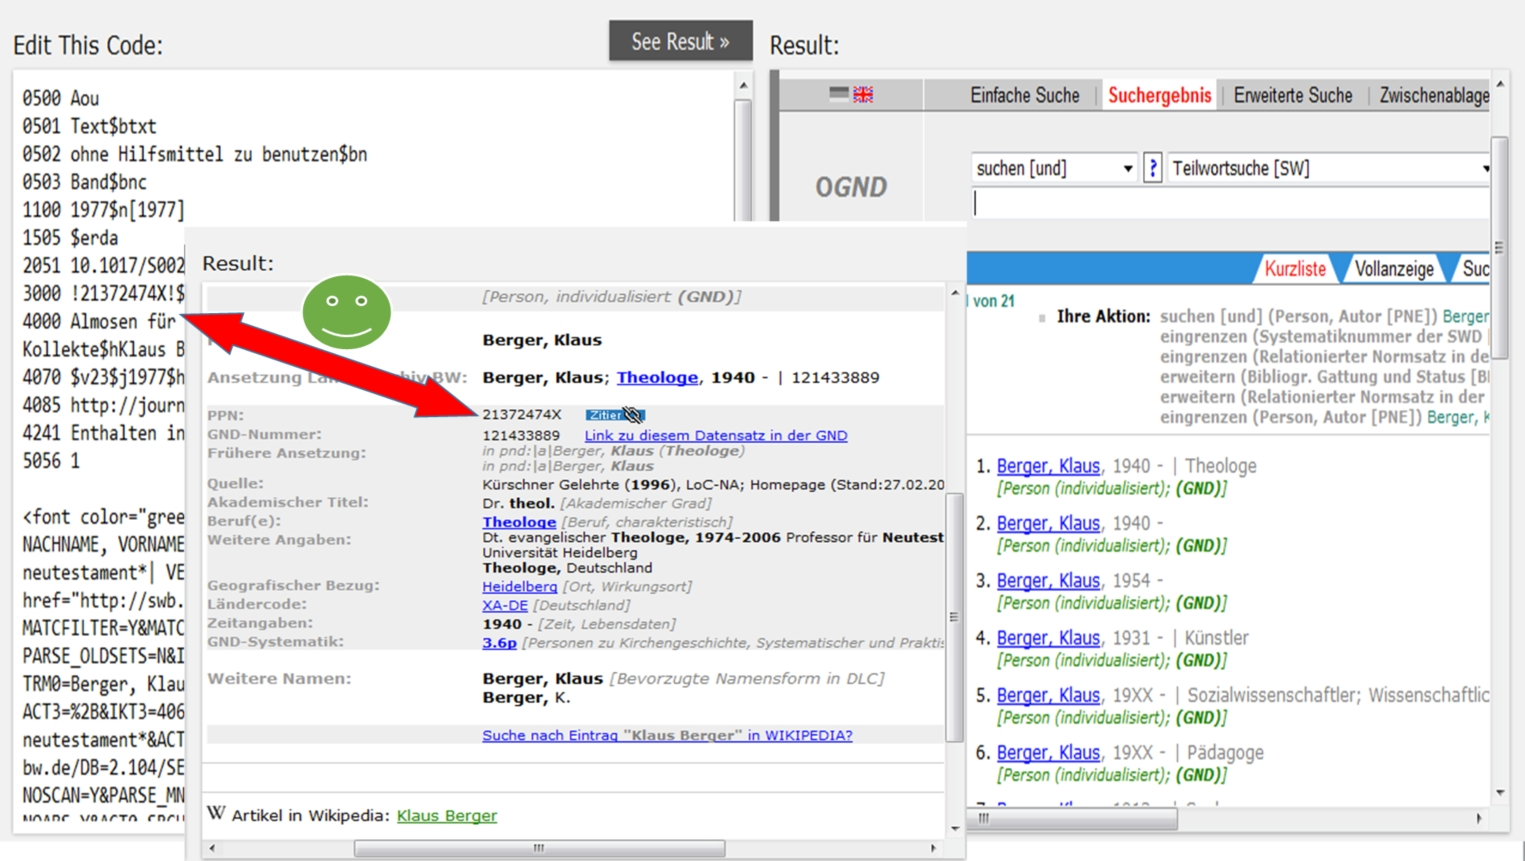
\includegraphics{img/Normdatenrecherche.jpg}
\caption{Normdatenrecherche rechts liefert einen eindeuten Theologen,
welcher mit der bereits automatisch gefundene PPN übereinstimmt}
\end{figure}

Damit wird Zotero hier als Vorstufe zum eigentlichen
Katalogisierungsclient geschaltet, die gesamte Bearbeitung findet
clientseitig statt und erlaubt auch noch weitere manuelle
Nachjustierungen im gewohnten Katalogisierungsumfeld der WinIBW. Vor
einigen Jahren gab es bereits einen Vorschlag im GBV (Voß 2008a; Voß
2008b), Zotero bei der Katalogisierung zu verwenden. Dabei wurde aber
vorgeschlagen Zotero als Katalogisierungsclient zu verwenden und einen
entsprechenden Webservice sowie Anbindungen an den Verbundkatalog
aufzusetzen. Dieses Vorhaben ist nicht weiter umgesetzt worden.

\section*{Zotero Pica3-Export-Translator im
Praxistest}\label{zotero-pica3-export-translator-im-praxistest}

Aufgrund der Verbesserungsvorschläge, die sich bei der Katalogisierung
während der Testphase ergaben, konnten wir für den Produktionsbetrieb
den Pica3-Export-Translator nach Katalogisierungsvorgaben weiter
ausbauen. So wurden beispielsweise folgende Anpassungen realisiert:
wiederholte Feldbelegung 30xx bei mehr als einem/r Verfasser/in,
Trennung des Untertitels vom Titel mit \enquote{\$d}, sprachspezifische
Umsetzung des Sortierzeichens \enquote{@} nach einem Artikel\footnote{\url{https://github.com/UB-Mannheim/zotkat/files/137992/ARTIKEL.pdf}}
und Anpassung unterschiedlicher Zeichensetzung zwischen Zotero-internem
Format und WinIBW-Format.

In vielen Fällen war es nach diesen Anpassungen möglich, die in Pica3
konvertierte Titelaufnahme ohne nachträgliche Bearbeitung in WinIWB
direkt -- ähnlich wie bei einer Datenübernahme über Broadcast-Search in
WinIBW -- abzuspeichern. Während der Testphase beschränkte sich die
nachträgliche Korrektur auf die Groß- und Kleinschreibung der
fremdsprachigen Titel, die mit dem Translator technisch nicht abgefangen
werden konnte. Diese Korrektur war während der Testphase im laufenden
Produktionsbetrieb auch deshalb notwendig, da die Aufsätze nach der
gedruckten Vorlage mit dem Katalogisierungsniveau \enquote{Aou}
(=Katalogisat der Druckausgabe nach Autopsie) erfasst wurden, während
die heruntergeladenen Metadaten der Online-Ausgabe bisweilen geringfügig
davon abwichen.

\section*{Retrospektive Erfassung der IxTheo-Zeitschriften vor
1976}\label{retrospektive-erfassung-der-ixtheo-zeitschriften-vor-1976}

Im Rahmen eines Projekts wurden Aufsätze aus Zeitschriftenarchiven der
National- und Allianzlizenzen\footnote{\url{https://www.nationallizenzen.de/angebote}}
nach Katalogisierungsniveau \enquote{Aor} (=Katalogisat ohne Autopsie)
beziehungsweise \enquote{Aon} (=maschinell konvertierte Katalogisate)
rückwärtig erfasst, so dass hier keine nachträgliche Korrektur an der
Titelaufnahme erforderlich war.

Lediglich die automatisch verknüpften Autoren-PPNs wurden in der OGND
überprüft und bei Nicht-Verknüpfung die Autoren gegebenfalls mit dem
oben dargestellten Verfahren manuell verknüpft. Wenn keine Normdaten zu
dem Autorennamen vorhanden waren, wurden die Namen als Text im
Autoren-Feld 30xx stehen gelassen und der Satz in \enquote{Aon}
geändert, um später im laufenden Betrieb nach Neuansetzung der Personen
durch geschultes Bibliothekspersonal verknüpft werden zu können. Zudem
wurde eine \enquote{Datenmaske} für ein lokales Abrufzeichen und die
IxTheo-Klassifikation im Exemplarsatz\footnote{\url{https://www.gbv.de/wikis/cls/WinIBW3:Datenmasken}}
angelegt, um sich Schreibarbeit zu ersparen. Da wir von Beginn an bei
der retrospektiven Katalogisierung das lokale Abrufzeichen
\enquote{ixzo} für Titel, die mit Zotero katalogisiert werden, vergeben
haben, konnten diese Titel in WinIBW leicht abgefragt und das
Testergebnis statistisch festgehalten werden:

\begin{longtable}[c]{@{}cccc@{}}
\caption{Ergebnistabelle (wird unten fortgesetzt)}\tabularnewline
\toprule
\begin{minipage}[b]{0.11\columnwidth}\centering\strut
ISSN
\strut\end{minipage} &
\begin{minipage}[b]{0.24\columnwidth}\centering\strut
Erfassungszeitraum
\strut\end{minipage} &
\begin{minipage}[b]{0.15\columnwidth}\centering\strut
Insgesamt
\strut\end{minipage} &
\begin{minipage}[b]{0.38\columnwidth}\centering\strut
(Vpos) mit Normdaten verknüpft
\strut\end{minipage}\tabularnewline
\midrule
\endfirsthead
\toprule
\begin{minipage}[b]{0.11\columnwidth}\centering\strut
ISSN
\strut\end{minipage} &
\begin{minipage}[b]{0.24\columnwidth}\centering\strut
Erfassungszeitraum
\strut\end{minipage} &
\begin{minipage}[b]{0.15\columnwidth}\centering\strut
Insgesamt
\strut\end{minipage} &
\begin{minipage}[b]{0.38\columnwidth}\centering\strut
(Vpos) mit Normdaten verknüpft
\strut\end{minipage}\tabularnewline
\midrule
\endhead
\begin{minipage}[t]{0.11\columnwidth}\centering\strut
0048-1009
\strut\end{minipage} &
\begin{minipage}[t]{0.24\columnwidth}\centering\strut
1956 - 1976
\strut\end{minipage} &
\begin{minipage}[t]{0.15\columnwidth}\centering\strut
392 Aufsätze
\strut\end{minipage} &
\begin{minipage}[t]{0.38\columnwidth}\centering\strut
240 Aufsätze nach \enquote{Aor} Prozentsatz: 61,22\%
\strut\end{minipage}\tabularnewline
\begin{minipage}[t]{0.11\columnwidth}\centering\strut
0028-6885
\strut\end{minipage} &
\begin{minipage}[t]{0.24\columnwidth}\centering\strut
1959 - 1977
\strut\end{minipage} &
\begin{minipage}[t]{0.15\columnwidth}\centering\strut
602 Aufsätze
\strut\end{minipage} &
\begin{minipage}[t]{0.38\columnwidth}\centering\strut
354 Aufsätze nach \enquote{Aor} Prozentsatz: 58 \%
\strut\end{minipage}\tabularnewline
\bottomrule
\end{longtable}

\begin{longtable}[c]{@{}cc@{}}
\toprule
\begin{minipage}[b]{0.34\columnwidth}\centering\strut
(Vnot) Nicht verknüpft
\strut\end{minipage} &
\begin{minipage}[b]{0.37\columnwidth}\centering\strut
Ergebnis
\strut\end{minipage}\tabularnewline
\midrule
\endhead
\begin{minipage}[t]{0.34\columnwidth}\centering\strut
152 Aufsätze nach \enquote{Aon} Prozentsatz: 38,78 \%
\strut\end{minipage} &
\begin{minipage}[t]{0.37\columnwidth}\centering\strut
16 h / 392 = ca. 2 ½ min pro Aufsatz inkl. Vergabe der IxTheo-Klassen
für Neues Testament im Lokalsatz
\strut\end{minipage}\tabularnewline
\begin{minipage}[t]{0.34\columnwidth}\centering\strut
248 Aufsätze nach ``Aon`` Prozentsatz: 42 \%
\strut\end{minipage} &
\begin{minipage}[t]{0.37\columnwidth}\centering\strut
30 h / 601 = ca.3 min pro Aufsatz inkl. Vergabe der IxTheo-Klassen für
Neues Testament im Lokalsatz
\strut\end{minipage}\tabularnewline
\bottomrule
\end{longtable}

Bei der nachträglichen Verknüpfung der Autorennamen stieg der Anteil von
\enquote{Vpos} auf circa 67\%.

Die Gründe für das Nicht-Verknüpfen waren zum einen, dass keine
Personensätze zu den Namen vorhanden waren, und zum anderen, dass die
Normdaten oft nur als Tni-/Tpi-Sätze existierten und nicht ausreichend
individualisiert waren.

Die Rückmeldung des Bibliothekspersonals waren nach der Testphase
insgesamt positiv, vor allem seien Ergonomie und Usability durch das
Zotero-Verfahren im Vergleich zum bisher angewendeten Copy \&
Paste-Verfahren bei der Erfassung eines Aufsatzes deutlich verbessert
worden und eine zusätzliche, noch deutlichere Arbeitserleichterung sei
durch den automatisierten und nachjustierbaren Autorenabgleich bewirkt
worden.

\section*{Zusammenfassung und
Ausblick}\label{zusammenfassung-und-ausblick}

Summa summarum scheint Zotero als vorgeschaltetes Tool in Kombination
mit dem Katalogisierungsclient WinIBW einen Mehrwert unter anderem bei
der Verknüpfung von Normdaten anzubieten. Durch flexibel programmierbare
Abfragen und integrierbare Mappinglisten in Zotero Translator kann den
Katalogisierern bei der Arbeitsroutine geholfen und die Arbeit
effizienter gestaltet werden. Solche Normdatenverknüpfungen bieten dann
unmittelbar für die Bibliotheksnutzer weitere Zusammenhänge wie etwa die
Suche nach Publikationen eines bestimmten Autors oder eine automatische
Verlinkung verschiedener Datenbankeinträge desselben Autors\footnote{\url{https://tools.wmflabs.org/persondata/index.php}}
über sogenannte BEACON-Dateien\footnote{\url{http://www.ixtheo.de/beacon/ixtheo.txt}},
wie zum Beispiel zwischen Wikipediaartikel und anderen
Online-Bibliographien. Allgemeiner kann man dies als weiteren
Informationsteil der LOD Cloud ansehen.

Die verschiedenen Schritte in dem hier beschriebenen semiautomatischen
Katalogisierungsworkflow können auch von unterschiedlichen Personen
durchgeführt werden. Vorstellbar ist eine Teilung in drei Teile:

\begin{enumerate}
\def\labelenumi{\arabic{enumi}.}
\item
  Sammeln der Artikeldaten mit Zotero,
\item
  Herstellen der Normdatenverknüpfungen,
\item
  Speichern in der Ver\-bund\-daten\-bank.
\end{enumerate}

Die Schritte 2) und 3) sind momentan verschränkt und erfordern meist
tiefergehendes bibliothekarisches Know-How. Dahingegen ist es
vorstellbar, dass zum Beispiel auch Forscher innerhalb eines Projektes
theologische Zeitschriften auswerten und die Aufsatzdaten mit Zotero
sammeln. Prinzipiell kann der Schritt 1) auch als Dateningest etwa von
Herausgebern einer Zeitschrift genutzt werden, um die Aufnahme dieser
Artikel im Index Theologicus anzustoßen. Dabei können diese Daten in
einer Zotero-Gruppe kollaborativ und auch ohne profunde
Katalogisierungskenntnisse gesammelt werden. Die Bibliothek könnte sich
dann auf die Normdatenerstellung, -verknüpfung und das Abspeichern in
der Ver\-bund\-daten\-bank konzentrieren. Es bleibt eine spannende Frage, wie
man den Katalogisierungsablauf für diese Aufsatzdaten softwaregestützt
und kollaborativ weiter optimieren kann, um die Quantität der Titel aber
auch die Erschließungstiefe hoch zu halten.

\section*{Quellenverzeichnis}\label{quellenverzeichnis}

Faßnacht, M. (2015). Index Theologicus. Presented at the 16.
BSZ-Kolloquium am 22. September 2015 in der Universität Stuttgart,
Stuttgart. Retrieved from
\url{http://nbn-resolving.de/urn:nbn:de:bsz:576-opus-12418}

Pfeffer, M. (2016, March). \emph{Open Source Software zur Verarbeitung
und Analyse von Metadaten}. Vortragsfolien presented at the 105.
Deutscher Bibliothekartag in Leipzig 2016 = 6. Bibliothekskongress /
Themenkreis 4: Wissen organisieren und erhalten / LIS-Workshop
(16.03.2016, 14:00-18:00, Vortragsraum 10), Leipzig. Retrieved from
\url{https://opus4.kobv.de/opus4-bib-info/frontdoor/index/index/docId/2449}

Voß, J. (2008a). \emph{Simple Web Cataloging with Zotero}. GBV.
Retrieved from
\url{https://www.gbv.de/wikis/cls/Datei:SimpleWebCatalogingWithZotero/_7.1.pdf}

Voß, J. (2008b, February). Zotero als Katalogisierungsclient --
Verbund-Wiki GBV {[}Wikiseite{]}. Retrieved April 3, 2016, from
\url{https://www.gbv.de/wikis/cls/Zotero/_als/_Katalogisierungsclient}

Zumstein, P., \& Stöhr, M. (2015). Zur Nachnutzung von bibliographischen
Katalog- und Normdaten für die persönliche Literaturverwaltung und
Wissensorganisation. \emph{ABI-Technik}, \emph{35}(4), 210--221.
\url{http://doi.org/10.1515/abitech-2015-0037}

Zur Geschichte des Index theologicus. (2007, January). Retrieved April
3, 2016, from \url{http://www.ixtheo.de/histger.htm}

%autor

\end{document}